\chapter{Introduction}

Let me introduce to the topic of my Masters work at \acrfull{sk}.


% 1. Introduction (10%) 1-1.5 pp

The project topic is related to the problem of human indoor navigation and positioning. 
The specified context states that no GPS data are available at hand, which makes the use of common navigation services impossible.

Most of existing indoor navigation systems require a special mapping stage. This is due to the reason we need to have a map for localization. A map usually consists of observations with recorded locations being organized in a special way.

Novel position systems can utilize the data recorded from users. This is called the crowd-source approach in positioning systems design. This approach makes the data collection cheaper and faster by orders. This allows to create a maps of public buildings and other locations, similar to Google maps or other products. These maps data are available online and several companies are working on this data collection specifically.

For real-time indoor navigation, in conditions where is no initial data is available, we have to perform multiple stages of localization and mapping. This can also be done simultaneously in SLAM approach. \\
We aim to utilize both SLAM and crowd-source approaches for the best performance of positioning system.

The innovation of this research is in ability to provide same navigation services with less information and in more natural way, which means also the reduced cost of the system overall.
Given paper focuses on implementation the data from magnetic field to localization and mapping framework. This technology choice is supported with additional technological research materials.

\section*{Motivation}

Indoor navigation is a market solving different problems with logistics inside buildings. The problem is important because more than $90 \%$ of time people usually spend inside the buildings \cite{IndoorGeneration}.

Time spent for logistics such as path choice, search for special places / people can't be measured, but we will agree that it's a wasted time.

Hundreds different applications, dozens of existing technologies, and no really perfect and universal solution. By word perfect we assume comparing to GPS - global, universal, precise enough for usual tasks, stable and free to people.

Existing technologies such as WiFi localization and others will be covered where possible, but the focus of paper is mostly on Indoor positioning as a product it should be: product with price, business plan, technology inside and with the need from customers.

Understanding the technology doesn't bring us to the product. There are different researches of positioning technologies\cite{Mautz2012IndoorPT, Sakpere2017ASS, Kj_fingerprinting, Brena2017}.
%We will focus on one use case, indoor positioning system for exhibitions.
% explain the scope of paper here
We have a vision of the product that is based on human localization in buildings. To develop this product we have to choose technology, methods, hardware and software if needed.
This part is covered specifically in Section \ref{cap:TechResearch}.

\section*{Terminology}

\begin{enumerate}
	\item [IPS ]- indoor positioning system
	\item [RTLS] - reat-time location service
	\item [BLE] - bluetooth low energy
\end{enumerate}


\section{Thesis Structure}

%The diagram in \autoref{fig:thesis-structure} illustrates the flow of information through the structure of the thesis.

%\begin{figure}[htb!]
%\centering 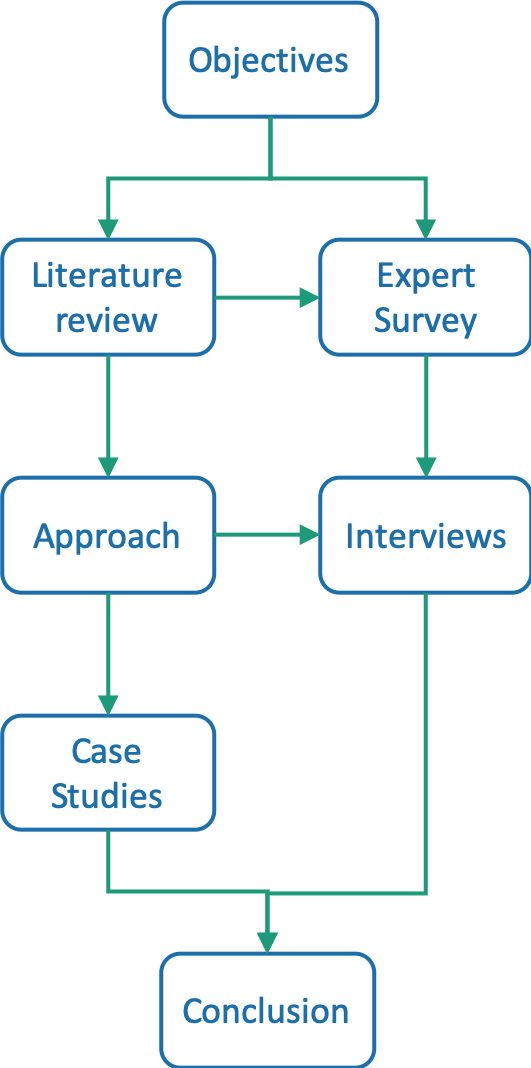
\includegraphics[width=0.5\textwidth]{graphics/thesis-structure}
%\caption{Thesis structure}
%\label{fig:thesis-structure}
%\end{figure}

% introduction
% 
% motivation
% state of the art systems
% system design & architecture
% 
% background, what is system, what features, how does it works
% data processing
% slam and graph minimization
% factor graphs, distance function, graph matching
% trajectory generation
% walking model
% 
% map construction
% observations to map (approximation, regressinon), map to observations (as a sensor)
% (sensor model), propagation model, slam / sam
% 
% conditioning on magnetic field data
% what graphs / figures can be plotted

\begin{description}
    \item[\Autoref{cap:background} - Background]
	The literature review and common concepts of the problem scope.
	Evaluation of current state-of-the-art approaches and technologies.

	\item[\Autoref{cap:TechResearch} - Techonogical research. ]
	Technological roadmap states various possible solutions to human indoor positioning problem. \\
	We develop a model for taking decision of technology / product choice; understanding physical limits. We highlight the landscape of related technologies.
	We use this model for technology choice and for the problem statement.

    \item[\Autoref{cap:thesis_objectives} - Thesis Objectives]
	We define the objectives of our work. Hypotheses we test and a system requirements.

	\item[\Autoref{cap:thesis_methodology} - Methodology]
	Methodology and ideas behind the research. Algorithms and experiments explained.

    \item[\Autoref{cap:conclusion} - Conclusion]
	Conclusion on our results we obtained.


\end{description}

